\documentclass[aps,prl,twocolumn,groupedaddress]{revtex4-1}
% \documentclass[aps,twocolumn,secnumarabic,balancelastpage,amsmath,amssymb,nofootinbib]{revtex4-1}
\usepackage{amsmath}
\usepackage{amssymb}
\usepackage{amsfonts}
\usepackage{color}
\usepackage{graphics}
\usepackage[pdftex]{graphicx}
\usepackage[utf8x]{inputenc}
\usepackage[colorlinks=true]{hyperref}

\newcommand{\ud}{\mathrm{d}}
\newcommand{\ue}{\mathrm{e}}
\newcommand{\ui}{\mathrm{i}}
\newcommand{\res}{\mathrm{Res}}
\newcommand{\Tr}{\mathrm{Tr}}
\newcommand{\dsum}{\displaystyle\sum}
\newcommand{\dprod}{\displaystyle\prod}
\newcommand{\dlim}{\displaystyle\lim}
\newcommand{\dint}{\displaystyle\int}
\newcommand{\fsno}[1]{{\!\not\!{#1}}}
\newcommand{\texp}[2]{\ensuremath{{#1}\times10^{#2}}}
\newcommand{\dexp}[2]{\ensuremath{{#1}\cdot10^{#2}}}
\newcommand{\eval}[2]{{\left.{#1}\right|_{#2}}}
\newcommand{\paren}[1]{{\left({#1}\right)}}
\newcommand{\lparen}[1]{{\left({#1}\right.}}
\newcommand{\rparen}[1]{{\left.{#1}\right)}}
\newcommand{\abs}[1]{{\left|{#1}\right|}}
\newcommand{\sqr}[1]{{\left[{#1}\right]}}
\newcommand{\crly}[1]{{\left\{{#1}\right\}}}
\newcommand{\angl}[1]{{\left\langle{#1}\right\rangle}}
\newcommand{\tpdiff}[4][{}]{{\paren{\frac{\partial^{#1} {#2}}{\partial {#3}{}^{#1}}}_{#4}}}
\newcommand{\tpsdiff}[4][{}]{{\paren{\frac{\partial^{#1}}{\partial {#3}{}^{#1}}{#2}}_{#4}}}
\newcommand{\pdiff}[3][{}]{{\frac{\partial^{#1} {#2}}{\partial {#3}{}^{#1}}}}
\newcommand{\diff}[3][{}]{{\frac{\ud^{#1} {#2}}{\ud {#3}{}^{#1}}}}
\newcommand{\psdiff}[3][{}]{{\frac{\partial^{#1}}{\partial {#3}{}^{#1}} {#2}}}
\newcommand{\sdiff}[3][{}]{{\frac{\ud^{#1}}{\ud {#3}{}^{#1}} {#2}}}
\newcommand{\tpddiff}[4][{}]{{\left(\dfrac{\partial^{#1} {#2}}{\partial {#3}{}^{#1}}\right)_{#4}}}
\newcommand{\tpsddiff}[4][{}]{{\paren{\dfrac{\partial^{#1}}{\partial {#3}{}^{#1}}{#2}}_{#4}}}
\newcommand{\pddiff}[3][{}]{{\dfrac{\partial^{#1} {#2}}{\partial {#3}{}^{#1}}}}
\newcommand{\ddiff}[3][{}]{{\dfrac{\ud^{#1} {#2}}{\ud {#3}{}^{#1}}}}
\newcommand{\psddiff}[3][{}]{{\frac{\partial^{#1}}{\partial{}^{#1} {#3}} {#2}}}
\newcommand{\sddiff}[3][{}]{{\frac{\ud^{#1}}{\ud {#3}{}^{#1}} {#2}}}

\begin{document}
\title{Motional Quantum Ground-State Cooing Outside the Lamb-Dicke Regime}
\author{Yichao Yu}
\author{Nicholas R. Hutzler}
\author{Jessie T. Zhang}
\author{Lee R. Liu}
\author{Kang-Kuen Ni}
\email{ni@chemistry.harvard.edu}
\affiliation{Department of Chemistry and Chemical Biology, Harvard University, Cambridge, Massachusetts, 02138, USA}
\affiliation{Department of Physics, Harvard University, Cambridge, Massachusetts, 02138, USA}
\affiliation{Harvard-MIT Center for Ultracold Atoms, Cambridge, Massachusetts, 02138, USA}

\date{\today}

\begin{abstract}
  Single neutral atom trapped in optical tweezer is a promising system for various applications
  in quantum information and simulation.
  The control of the motional states for such a system is crucial
  for exploiting its full potential.
  We report Raman sideband cooling of a single sodium atom to its three-dimensional
  motional ground state in an optical tweezer.
  Despite having a very large Lamb-Dicke parameter, high initial temperature and
  large differential AC Stark shift in the excited state,
  we achieved a ground state preparation fidelity of $77(4)\%$ after a few hundred ms of cooling
  by using a few new cooling techniques including addressing high order Raman sideband.
  We demonstrate that Raman sideband cooling to the 3D motional ground state is applicable to
  systems where tight confinement or low initial cooling is hard to achieve.
  The is particularly relevant for systems which are challenging to laser-cool,
  such as molecules and exotic atoms, and opens up a new approach for further cooling
  of these systems.
\end{abstract}

\maketitle

\begin{figure*}
  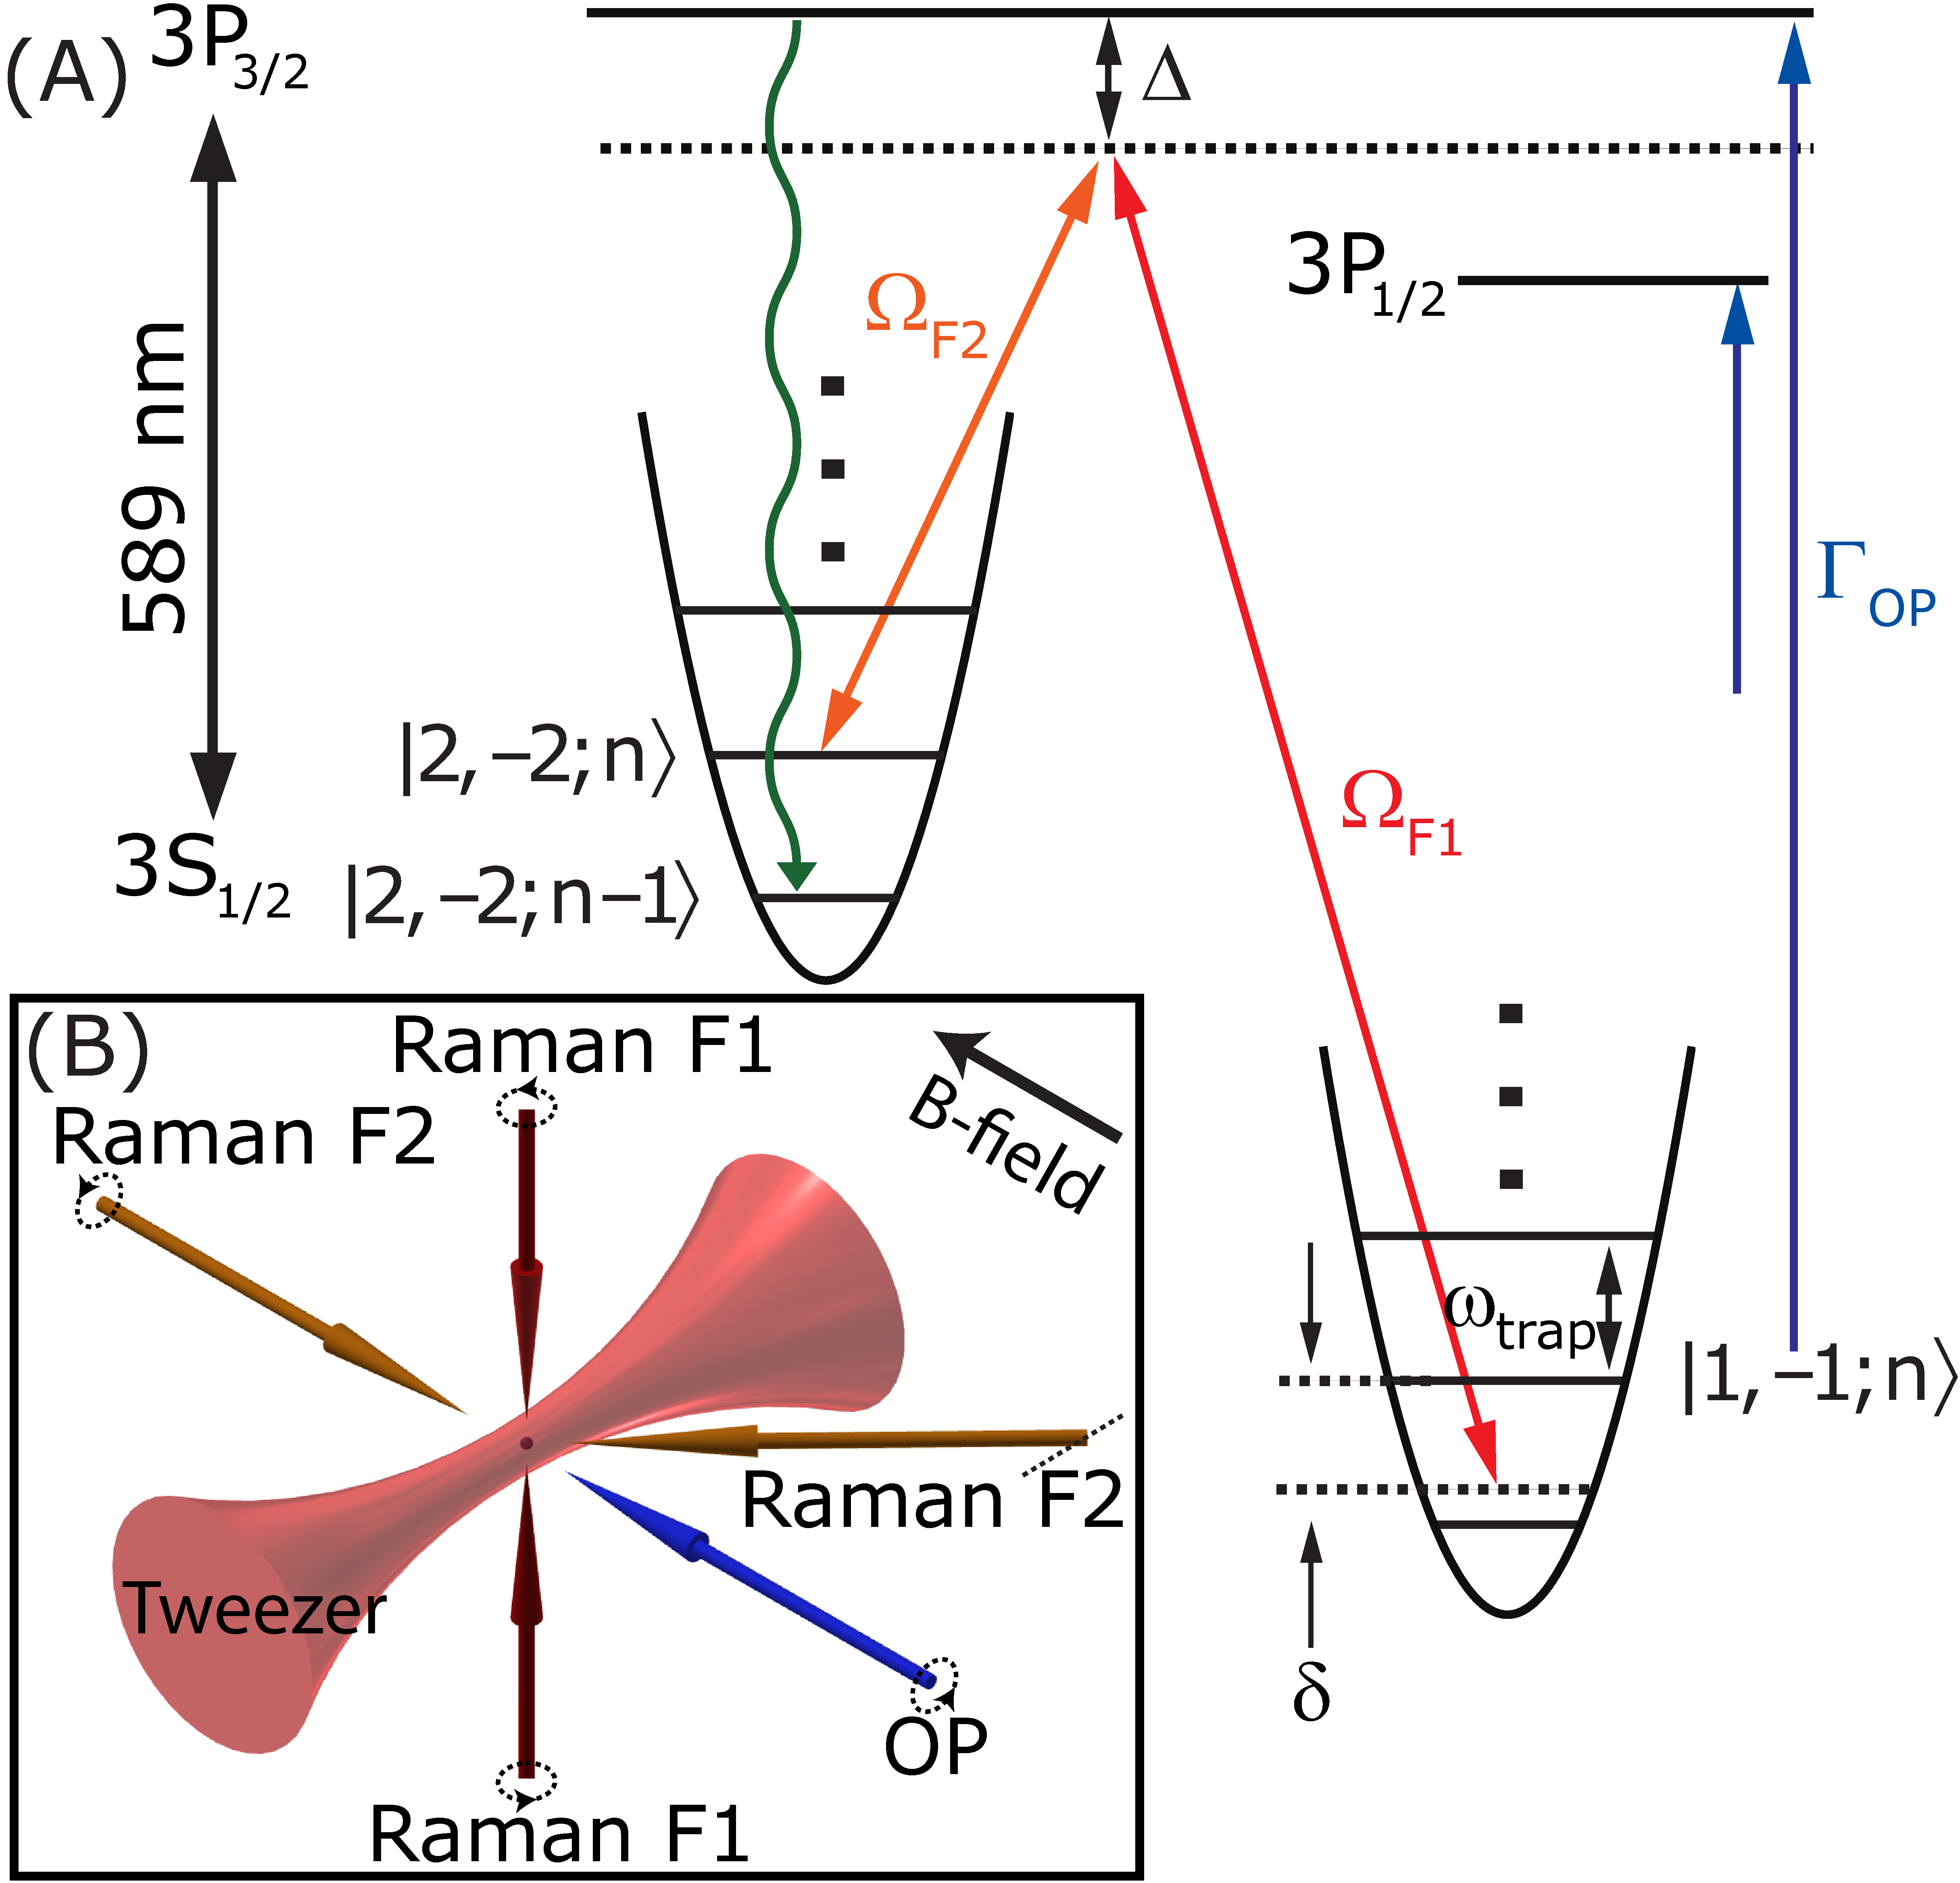
\includegraphics[height=5.2cm]{imgs/Na_RSC_schematic.pdf}
  \includegraphics[height=4.5cm]{sequence.pdf}
  \caption{(A) Energy levels and schematics of Raman sideband cooling.
    The Raman transitions has a one photon detuning $\Delta=25GHz$ from the D2 line.
    We use D1 light with $\sigma^-$ polarization to repump atom out of $|F=2,m_F=-1\rangle$
    state to minimize heating on the atom in $|F=2,m_F=-2\rangle$ state.
    (B) Geometry and polarizations of the Raman and optical pumping beams relative to the
    optical tweezer and bias magnetic field.
    (C) Schematics of the cooling sequence. The tweezer is switching at $3\text{MHz}$ to
    reduce light shift during optical pumping. Each cooling cycle consists of $8$ pulses.
    The four axial pulses are addressing two neighboring cooling orders.
    The two pulses in each radial directions are either addressing two neighboring cooling orders
    or having different length on the first order when most of the population are below $n=3$
    towards then end of the cooling sequence.
    \label{f-setup}}
\end{figure*}
\begin{figure}[b]
  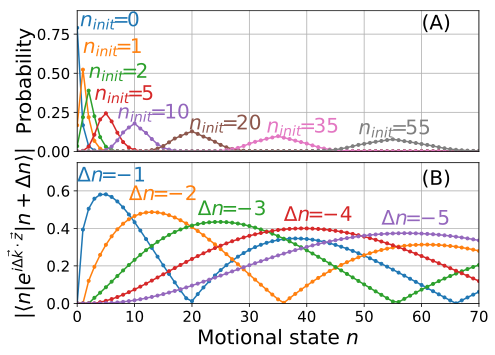
\includegraphics[width=8.5cm]{imgs/fig2_raman_op.pdf}
  \caption{Matrix elements and heating probabilities as a function of motional state.
    The range plotted covers $99\%$ of the initial thermal distribution.
    (A) Matrix elements for Raman transition in the axial direction showing deviation from
    $\sqrt{n}$ scaling and multiple minimums for different sideband orders.
    (B) Heating probability during the optical pumping step for all three axis.
    Due to the large Lamb-Dicke parameter,
    there is a high probability of heating especially in the axial direction.
    \label{f-ld}}
\end{figure}
\begin{figure*}
  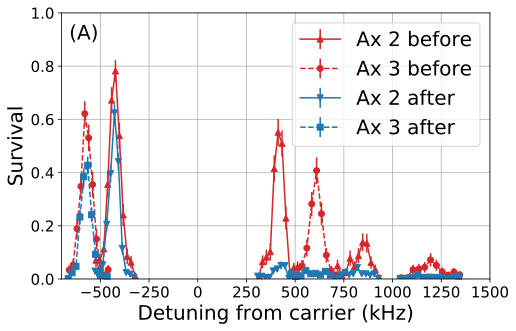
\includegraphics[height=4.2cm]{imgs/spectrum_r.pdf}
  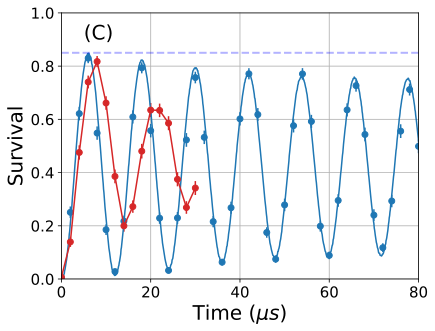
\includegraphics[height=4.2cm]{imgs/rabi_flop_r3_0.pdf}
  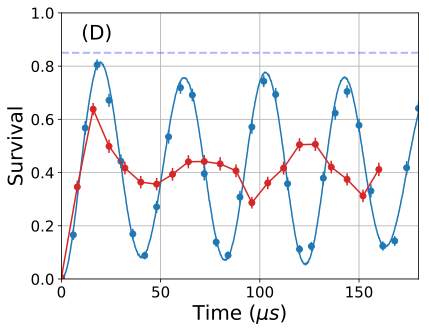
\includegraphics[height=4.2cm]{imgs/rabi_flop_r3_p1.pdf}
  \caption{Radial Raman sideband spectrum of first order heating, first order cooling and
    second order cooling (A) before and (B) after Raman sideband cooling.
    Rabi flopping on axis 3 (C) carrier and (D) first order heating sideband
    after cooling.
    Solid lines in (C) and (D) are theoretical fit with a ground state probability of $93\%$.
    \label{f-radial}}
\end{figure*}
\begin{figure*}
  \includegraphics[height=4.2cm]{imgs/spectrum_a1.pdf}
  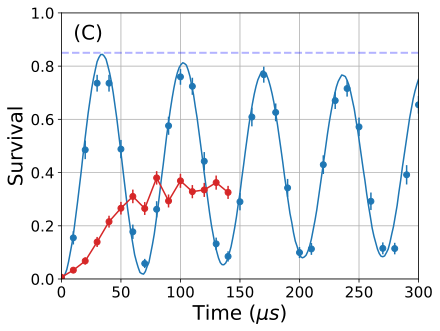
\includegraphics[height=4.2cm]{imgs/rabi_flop_a1_0.pdf}
  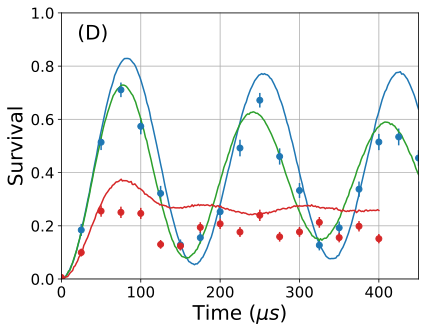
\includegraphics[height=4.2cm]{imgs/rabi_flop_a1_p1.pdf}
  \caption{Axial Raman sideband spectrum from first order heating to eighth order cooling
    (A) before and (B) after Raman sideband cooling.
    The data for the second and higher orders of cooling sidebands are taken with $150\mu s$
    pulse time and the rest are taken with $125\mu s$ pulse time.
    Rabi flopping on axial (C) carrier and (D) first order heating sideband
    after cooling.
    Solid lines in (C) and (D) are theoretical fit with a ground state probability of $92\%$.
    \label{f-axial}}
\end{figure*}

Systems of single neutral atoms trapped in optical tweezers are an exciting platform to study quantum information, quantum chemistry,
and quantum simulation of many-body systems [REF].
This approach provides full single-site resolution and control, and can feature long-range interactions via Rydberg atoms,
polar molecules, or dipolar atoms [REF].
Polar molecules in particular offer the additional advantages of long-lived internal states and a high degree of tunability,
including the shape, range, and strength of the interaction [REF].
Optical tweezers can also be re-arranged in real-time, allowing rapid preparation of atoms in complex geometries with high fidelity [REF].

In order to achieve long coherence times and full quantum control of the system,
it is typically necessary to cool the atom to the
three dimensional motional ground state in the optical tweezer.
This has been demonstrated for neutral Rb and Cs [REF] in experiments that had low initial temperature and small Lamb-Dicke parameter.  
These features
may not be easily achievable for other systems, such as directly laser-cooled polar molecules [REF],
or atoms with challenging sub-Doppler cooling such as Na, K, and Li [REF].
In this letter, we cool single sodium atoms
trapped in optical tweezers to the motional ground state with Raman sideband cooling.
Despite having a large Lamb-Dicke parameter and high initial temperature, we are able to achieve a ground state probability of $77(4)\%$
by utilizing several new cooling techniques and a carefully optimized cooling sequence.  Our approach is quite general, and opens up ground-state cooling for other systems.

The Raman sideband cooling (RSC) scheme that we use to achieve high ground state preparation fidelity
consists of multiple cycles of laser pulses to manipulate both the internal and
motional states of the atoms.
Figure \ref{f-setup}A shows the schematic of the energy levels and the cooling sequence
in our setup.
Each cooling cycle begins with the sodium atom in the $|F=2, m_F=-2\rangle$
ground electronic state and a certain vibration state $n$.
In the first step, a Raman pulse drives a transition to the motional state $n-\Delta n$
to reduce the motional energy while also changing the internal state to $|F=1, m_F=-1\rangle$.
In the second step, which finishes the cooling cycle,
<<<<<<< HEAD
an optical pumping pulse bring the atom back to the $|F=2, m_F=-2\rangle$ state.
The second step could also change the motional state of the atoms, which
could result in heating. The possibility for this to happen for an atom in the motional level $n$
is approximately proportional to the effective Lamb-Dicke (LD) parameter
$\eta^{OP}_{ef\! f}=\sqrt{2n+1}\eta^{OP}$ where $\eta^{OP}=???$ is the LD parameter for
optical pumping.
The geometry of the relevant beams (??? and their polarizations) is shown in figure \ref{f-setup}B.
=======
an optical pumping pulse bring the atom back to the $|F=2, m_F=-2\rangle$ state to take away
the entropy. The second step could also change the motional state of the atoms which
could cause heating. The possibility for this to happen for an atom in the motional level $n$
is approximately proportional to the effective Lamb-Dicke parameter
$\eta^{OP}_{eff}=\sqrt{2n+1}\eta^{OP}$ where $\eta^{OP}=k^{OP}\sqrt{\hbar/2m\omega}$ is the Lamb-Dicke parameter for
optical pumping.
The geometry of the relevant beams and their polarizations is showed in figure \ref{f-setup}B.
>>>>>>> refs/remotes/origin/master
The optical tweezer has one weakly confined axial direction (axis $1$) and
two more strongly confined radial directions (axis $2$ and $3$).
Multiple pairs of beams are used to drive the Raman transition during cooling in order to
isolate and maximize the coupling to different trap axes, each of which is independent and must be cooled individually.

<<<<<<< HEAD
Although RSC to the motional ground state has already been successfully
implemented in heavier neutral atoms like Rubidium [????]
and Cesium [????], such experiments generally use combine efficient sub-Doppler cooling
with tight confinement to achieve small LD parameters.
Since sub-Doppler cooling is challenging with sodium atoms, we begin the cooling sequence with a considerably larger LD parameter.  However, since these challenges will likely present themselves in other interesting systems like directly laser cooled molecules, the techniques we use to overcome these challenges will be useful for a wide variety of systems.

BRIEFLY DESCRIBE NA TRAPPING SETUP.

%As mentioned previously, in order to perform RSC efficiently and
%minimize the heating during the optical pumping, we need to have a small LD parameter, which for an optical tweezer means a low atom temperature. However, since the LD parameter $\eta$ is inversely
%proportional to $\sqrt{m}$ (???) where $m$ is the mass of the atom, it is larger for sodium
%given the same trap depth (???).

With 45 mW of power at the in the trap, we measure trapping frequencies of
$\{\omega_1,\omega_2,\omega_3\}/2\pi = \{67, 420, 580\}\ \text{\text{kHz}}$
which correspond to optical pumping LD parameters of
$\{\eta^{OP}_1,\eta^{OP}_2,\eta^{OP}_3\} = \{???, ???, ???\}$.
Moreover, due to hyperfine structure in the $3^2P_{3/2}$ manifold,
the sub-Doppler cooling in sodium is also less efficient and we start the
RSC with a initial temperature of $40\mu K$. Combined with the high LD
parameters, this gives us a initial effective optical pumping LD parameters of
$\{\eta^{OP}_{1eff},\eta^{OP}_{2eff},\eta^{OP}_{3eff}\} = \{???, ???, ???\}$
As a result, there is a very high probability of heating during each optical pumping step
(figure \ref{f-ld}B), resulting in a $30\%$ average heating probability during optical pumping
in the weakly-confined axial direction. 

Fortunately, the high LD parameters also
provide us with tools to overcome this issue. From our geometry, the LD parameters for
Raman transitions are $\{\eta^R_{1},\eta^R_{2},\eta^R_{3}\} = \{???, ???, ???\}$. As shown in
figure \ref{f-ld}A, this results in a strong coupling to higher orders
=======
Although Raman sideband cooling to motional ground state has already been successfully
implemented on neutral atoms in other experiments using heavier species like Rubidium
\cite{Thompson2013,Kaufman2012}
and Cesium [??], such experiments generally use good polarization gradient cooling
and a tight confinement to achieve a small Lamb-Dicke parameter and effective Lamb-Dicke parameter.
However, this regime is harder to achieve with sodium atoms, creating additional challenges for
us to realize ground state cooling. On the other hand, since these conditions can also be difficult
to meet for other interesting systems like directly laser cooled molecules, the techniques we
use to overcome these challenges could be useful for a wider variety of systems.

As mentioned previously, efficient Raman sideband cooling to the 3D ground state has been achieved in systems with
low initial temperature and
 small Lamb-Dicke parameter. However, since the Lamb-Dicke parameter $\eta$ is inversely
proportional to $\sqrt[4]{m}/\lambda$ where $m$ is the mass of the atom and $\lambda$
is the wavelength of the atomic transition,
it is larger for sodium given the same trap depth due to its low mass and short D line wavelength.
With 45 mW of power at the focus of the trap, we measured a trapping frequency of
$\{\omega_1,\omega_2,\omega_3\}/2\pi = \{69, 430, 590\}\ \text{\text{kHz}}$
which corresponds to optical pumping Lamb-Dicke parameters of
$\{\eta^{OP}_1,\eta^{OP}_2,\eta^{OP}_3\} = \{0.60, 0.24, 0.21\}$.
Moreover, due to the small hyperfine structure in the $3^2P_{3/2}$ manifold,
the sub-Doppler cooling in sodium is also less efficient and we start the
Raman sideband cooling with a initial temperature of $70\mu K$. Combined with the high Lamb-Dicke
parameters, this gives us a initial effective optical pumping Lamb-Dicke parameters of
$\{\eta^{OP}_{1eff},\eta^{OP}_{2eff},\eta^{OP}_{3eff}\} = \{3.97, 0.67, 0.50\}$
As a result, there is a very high probability of heating during the optical pumping step
(figure \ref{f-ld}B) causing a $30\%$ average heating probability during optical pumping
in the weakly confined axial direction. Fortunately, the high Lamb-Dicke parameters also
provide us tools to overcome this issue. From our geometry, the Lamb-Dicke parameters for
Raman transitions are $\{\eta^R_{1},\eta^R_{2},\eta^R_{3}\} = \{0.40, 0.34, 0.29\}$. As shown in
figure \ref{f-ld}A, the high Raman Lamb-Dicke parameters causes a strong coupling to higher orders
>>>>>>> refs/remotes/origin/master
of cooling sidebands, especially for high motional states.
This enables us to cool atoms in high motional states by driving on higher order Raman sidebands,
thereby removing more motional energy in a single cooling pulse and offsetting the effect of
additional heating. Since the heating probability is higher for high motional states,
cooling on these high order sidebands can greatly suppress the high heating during
optical pumping during the initial cooling. 

As shown in Figure \ref{f-ld}, the relationship between coupling strength, sideband order, and motional state is complicated.  There are also motional states where the coupling vanishes, providing an accumulation point for cooling processes that use a fixed sideband order, and halting cooling.  By using multiple orders of motional sidebands for the cooling cycles, we can avoid these accumulation points and achieve high efficiency cooling.

The large Raman LD parameters $\eta^R$
also create difficulties for measuring the temperature. Traditional sideband thermometry relies on
a relationship between the cooling/heating sideband heights and $\bar n$ that is only valid in the regime where the LD is small. However, since we are not in this regime, the coupling strength deviates from this simple scaling rule quickly as already
shown in figure \ref{f-ld}A, causing the normal sideband thermometry to break down.
In order to solve this problem, when the atom temperature is still high,
we measure the heights of multiple sidebands to make sure no population is hidden at the
minimum of one sideband order [THIS NEEDS TO BE EXPLAINED MORE CLEARLY]. After the atom is cooled and only occupies a small number of motional states, the LD approximation becomes valid.
This result is then verified using independent measure of Rabi flopping on the carrier and heating
sidebands since they provide more information about the distribution of coupling strength.

Another issue caused by the high initial temperature is trap anharmonicity.
Although the potential near the center of a focused Gaussian beam can be approximated
by a harmonic trap, when a large number of levels are populated due to high initial temperature
the anharmonicity of the trap can lead to broadening of the sideband and decrease of
the sideband signal. In our setup, this limits the Rabi frequency of the Raman pulse
on the radial sidebands to be no lower than tens of kiloHertz in order to drive atoms in
different motional states equally. [EXPLAIN THIS FURTHER]

Finally, the deep trap that is needed to trap and image single sodium atom also creates
a very large AC Stark shift in the excited state. For the trap depth we are using, the
light shift in the center of the trap is as large as $300\text{MHz}$.
In addition to creating a large and position dependent detuning for the optical pumping light,
it also mixes the excited state state hyperfine levels,
affecting the branching ratio and increasing the number of photons needed during optical pumping.
<<<<<<< HEAD
Similar to our loading and imaging process [???], we solve this issue by modulating the
tweezer at $3\text{MHz}$ during the whole cooling sequence.
=======
Similar to our loading and imaging process \cite{Hutzler2016},
we solve this issue by switching the trapping light at $3\text{MHz}$
during the whole cooling sequence.
>>>>>>> refs/remotes/origin/master
Due to the large light shift, the optical pumping is effectively off when the trap light is on.
Since the atom can only be addressed by the optical pumping light when the trap light is off,
the effect of light shift on optical pumping fidelity is suppressed.

Taking all the features of our system into account, we use a Monte-Carlo simulation to verify
the validity of our method.
In the simulation, we can observe the high heating rate due to the high LD parameters
and confirm our cooling sequence we can
overcome this effect and cool the atom successfully.
The simulation is also used to guide the optimization of the cooling sequence by exploring the
large parameter space and finding a robust cooling strategy. As shown in figure \ref{f-setup}B,
we found that instead of cooling on only one sideband order at a time, it is generally more
efficient to alternate the cooling pulse between two neighboring orders (axial) or pulse lengths.
A cooling sequence like this minimizes the accumulation of atom in a state not addressed by a
particular Raman pulse parameter.

For the more tightly confined radial directions,
<<<<<<< HEAD
we begin the cooling with $\{\bar n_2, \bar n_3\}=????, ????$.
=======
we starts the cooling with $\{\bar n_2, \bar n_3\}=2.2, 1.9$.
>>>>>>> refs/remotes/origin/master
The radial sideband spectra of the initial distribution is shown in figure \ref{f-radial}A
where we can clearly see the first order heating, first order cooling and
second order cooling sidebands.
The results of applying approximately 1000 cooling cycles in all three dimensions,
starting with the radial second order sideband,
are shown in figure \ref{f-radial}B,
where the first and second order cooling sidebands on both axes are suppressed.
Given the absence of the second order cooling sideband,
we can estimate the ground state probability in each direction based on the height of
the first order cooling and heating sideband to be $89.7(19)\%$ and $93.8(26)\%$.
Due to the complexity of the sideband structure,
we measured the Rabi flopping on the carrier and heating sideband before and after cooling
(\ref{f-radial}C and \ref{f-radial}D)
as a independent way to obtain the population in different motional states.
Fitting the Rabi flopping data give a ground state probability of $90\%$ and $92\%$,
showing good agreement between the two methods.
<<<<<<< HEAD
\begin{figure*}
  \includegraphics[height=4.3cm]{imgs/spectrum_a1.pdf}
  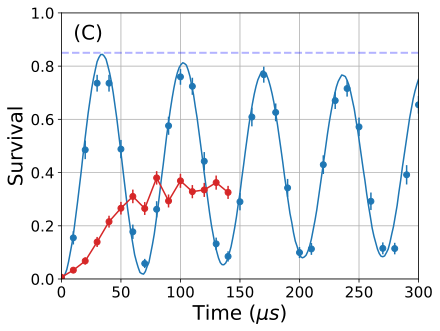
\includegraphics[height=4.3cm]{imgs/rabi_flop_a1_0.pdf}
  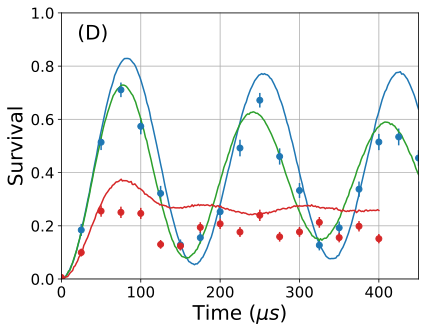
\includegraphics[height=4.3cm]{imgs/rabi_flop_a1_p1.pdf}
  \caption{Axial Raman sideband spectrum from first order heating to eighth order cooling
    (A) before and (B) after RSC.
    Rabi flopping on axial (C) carrier and (D) first order heating sideband
    after cooling.
    Solid lines in (C) and (D) are theoretical fit with a ground state probability of $????\%$.
    Horizontal dashed lines in (C) and (D) are total survival and detection efficiency.
    \label{f-axial}}
\end{figure*}

The axial direction is much less confined and therefore has a much higher initial effective
LD parameter of $\eta^{OP}_{eff1}\approx3.3$.
The line in figure \ref{f-axial}A shows the Raman spectrum in the axial direction
before applying RSC, where we can see clearly resolved sidebands
up to the eighth order, suggesting that we have many motional states populated in this direction.
Therefore, we begin our cooling sequence by driving Raman transitions on the eighth order axial
cooling sideband. After applying a cooling sequence similar to that used to cool
the radial directions, we obtain the spectrum shown in figure \ref{f-axial}B.
All of the higher order ($\geqslant2$) axial cooling sidebands disappear, and the first order
cooling sideband is strongly suppressed.
The ground state probability calculated from this spectrum is $????$.
=======

The axial direction is much less confined and therefore has a much higher initial effective
Lamb-Dicke parameter of $\eta^{OP}_{eff1}\approx3.97$.
The line in figure \ref{f-axial}A shows the Raman spectrum in the axial direction
before applying Raman sideband cooling where we can see clearly resolved Raman cooling sidebands
up to the eighth order suggesting that we have many motional states populated in this direction.
Therefore, we starts our cooling sequence by driving Raman transitions on the eighth order axial
cooling sideband. After applying the cooling sequence identical to the one we use to cool
the radial directions, the spectrum is shown in figure \ref{f-axial}B.
All of the high order ($\geqslant2$) axial cooling sidebands disappeared and the first order
cooling sideband is also strongly suppressed.
The ground state probability calculated from this spectrum is $91.6(28)\%$.
>>>>>>> refs/remotes/origin/master
We can also use Rabi flopping on the carrier and heating sideband to verify this result
similar to the radial direction. In this case, we see very good agreement on the carrier
(figure \ref{f-axial}B) but there is additional decoherence on the axial first order
heating sideband (figure \ref{f-axial}C).
We believe this decoherence is caused by technical noise in our setup which
produces the strongest effect on this transition due to its slow Rabi frequency.
The decoherence time scale agree with the magnetic field fluctuation we measured which produces
a Zeeman shift of around $5\text{kHz}$.

Combining the axial and radial cooling results,
we have achieved a ground state probability of $77.1(35)\%$.
We believe this is currently limited by off-resonant scattering from the Raman beams
and the resonance shift caused by magnetic field fluctuation.
<<<<<<< HEAD
Improvements on these should improve the cooling performance even further.  [EXPAND ON THIS]
=======
Improvements on these should improve the cooling performance even further.
We have shown that despite the difficulty in cooling sodium atoms,
it is possible to achieve reliable three dimensional cooling with significant ground state
probability using new cooling techniques and a optimized cooling sequence.
This opens up the possibility of cooling a large variety of systems to their motional ground
state using Raman sideband cooling that is challenging to laser cool
including molecules and exotic atoms.
>>>>>>> refs/remotes/origin/master

% Missing:
% ?? Blackman pulse vs square pulse

\bibliography{paper}
\end{document}
